\setchapterpreamble[u]{\margintoc}
\chapter{Autovalori e autovettori}
\labch{eigenvalues}

\section{Introduzione ed esercizio 8}

\subparagraph{File necessari} \texttt{eigenvalues.hpp}

\subparagraph{Esercizio}

Per illustrare esaustivamente le tecniche numeriche utilizzate si considerino i
vari punti dell'esercizio 8 partendo dalla matrice seguente:

\[ A = \begin{pmatrix}
		4 & -i   & 2    \\
		i & 2    & 2+7i \\
		2 & 2-7i & -2
	\end{pmatrix} \]

\section{Punto 1: Power method}

\paragraph{Nozioni teoriche}

Il primo metodo e' definito \textit{Power method} e consiste nel calcolare l'autovalore piu' grande di una matrice $A$ e l'autovettore associato.

Dato un qualsiasi vettore per il teorema spettrale se $A$ e' diagonalizzabile allora ogni vettore $\mathbf{x}_0$ puo' essere scritto sulla base dagli autovettori $\mathbf{v}_n$ di $A$.

Prendiamo dunque il vettore:

\[ \mathbf{y}_n = \mathbf{A}^n \mathbf{x}_0 = \sum_m^N c_m \lambda_m^n \mathbf{v}_m= \lambda_{max} \sum_m^N c_m \left( \frac{\lambda_m}{\lambda_{max}} \right)^n \mathbf{v}_m\]

Per numeri sufficientemente grandi di $N$ e se il rapporto $\frac{\lambda_m}{\lambda_{max}}$ e' minore di 1 allora il termine $\left( \frac{\lambda_m}{\lambda_{max}} \right)^n$ tende a 0 e quindi il termine dominante e' $\lambda_{max}$.

Quindi \[ \lim_{n \rightarrow \infty} \mathbf{y}_n = c_0 \lambda_{max} \mathbf{v}_0 \]

Visto che $\mathbf{y}_0$ e' multiplo di $\mathbf{v}_0$ esso stesso e' autovettore .

Per ottenere l'autovalore calcoliamo il cosiddetto \textit{Coefficiente di Rayleigh}

\[ \mathsf{C}_R = \frac{\mathbf{y}_n^T \mathbf{A} \mathbf{y}_n}{\mathbf{y}_n^T \mathbf{y}_n} \xrightarrow{n = \infty} \frac{\mathbf{v}_0^T \lambda_{max} \mathbf{v}_0}{\mathbf{v}_0^T \mathbf{v}_0} = \lambda_{max} \]

\subparagraph{Shifted Power Method}

Per casi particolari (principalmente autovalori simmetrici e opposti, come si vedra' nella ricerca degli zeri di polinomi ortonormali) si utilizza il \textit{Shifted Power Method}: si introduce uno shift $A + \alpha I$ per rendere lo spettro positivo e si reshiftano gli autovalori di $\lambda-\alpha$ ad algoritmo finito. Questo evita il carattere oscillatorio che si puo' estaurare quando $\lambda_i = -\lambda_j$.
In questo capitolo assumeremo $\alpha = 0$.

\paragraph{Implementazione}

La documentazione dell'algoritmo e' esaustiva e non necessita di ulteriori spiegazioni.

\paragraph{Risultati} si ottiene il seguente output:

\begin{lstlisting}
Power Eigenvalue: (8.45188,-2.22045e-16)
Power Eigenvector: 
 (0.387073,-0.143579)
 (0.350492,0.615922)
 (0.55364,-0.144353)

Ax= 
 (0.387073,-0.143579)
 (0.350492,0.615922)
 (0.55364,-0.144353)
\end{lstlisting}

Dove tra parentesi si indica la parte reale e immaginaria rispettivamente, inoltre il metodo funziona correttamente visto che $Ax = \lambda x$ ($\lambda$ e' molplicato nell'autovettore ma essendo una costante cio' e' ininfluente).

\section{Punto 2: Inverse Power method}

\paragraph{Nozioni teoriche}

Analogamente per il metodo precedente si puo' calcolare l'autovalore piu' piccolo di una matrice $A$ e l'autovettore associato, in questo caso si invertira' $A$e si raccogliera' il termine piu' piccolo $\lambda_{min}$ mentre $\left( \frac{\lambda_{min}}{\lambda_n} \right)^n \rightarrow 0$, lo stesso ragionamento si puo' anche fare per lo shift in questo caso esso verra' utilizzato per raggiungere piu' velocemente il risultato.

\paragraph{Risultati} Si ottiene:

\begin{lstlisting}
 Inverse Power Eigenvalue: (3.1896,-6.93889e-18)
Inverse Power Eigenvector: 
 (0.00850804,0.906366)
 (0.370705,-0.0809101)
 (0.0370076,-0.181906)

Ax= 
 (0.00850804,0.906366)
 (0.370705,-0.0809101)
 (0.0370076,-0.181906)
\end{lstlisting}

Il risultato e' inoltre verificato dal controllo di $\mathbf{Ax}$.

\section{Punto 3: studio della convergenza}

\paragraph{Risultati}


\begin{marginfigure}
	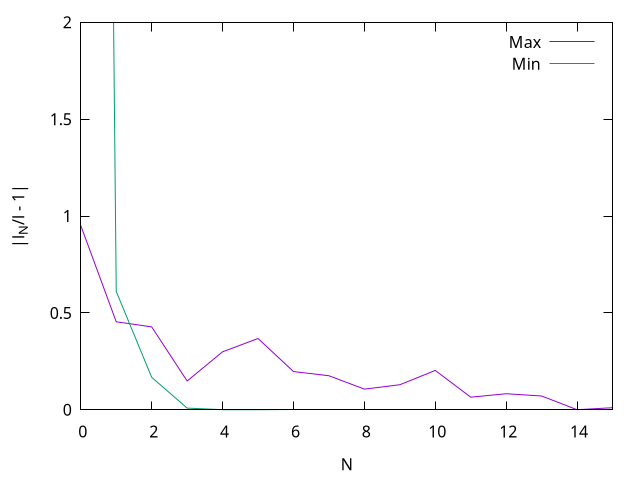
\includegraphics[width=1.5\textwidth]{eigen_convergence.png}
	\caption{Confronto tra la velocita' di convergenza dei due metodi}
	\label{fig:eigenconv}
\end{marginfigure}

Il risultato e' visibile nella figura \ref{fig:eigenconv}.

\paragraph{Analisi e conclusioni}

\begin{marginfigure}
	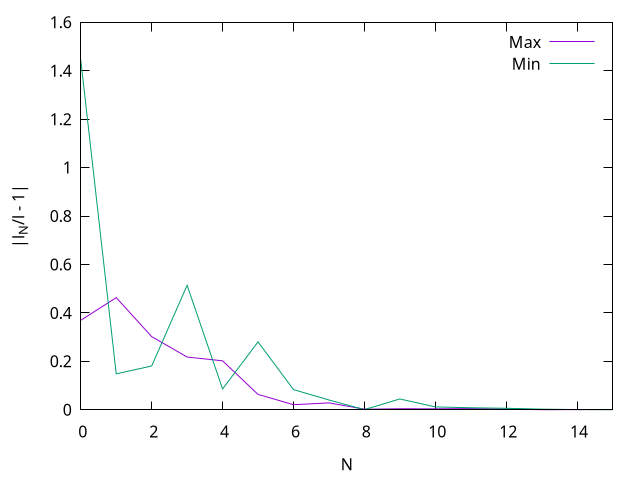
\includegraphics[width=1.5\textwidth]{eigen_convergence_2.png}
	\caption{Confronto tra la velocita' di convergenza dei due metodi, con $a_{00} = 8$}
	\label{fig:eigenconv_2}
\end{marginfigure}


Come si puo' osservare il metodo inverso converge molto piu' velocemente del
metodo diretto. Questo pero' dipende dagli autovalori della matrice e dal
rapporto $\lambda_n/\lambda_{max}$ e $\lambda_{min}/\lambda_n$. Per esempio,
presa la matrice A con $a_{00} = 8$ gli autovalori sono molto piu' vicini e si
ottiene la figura \ref{fig:eigenconv_2}.

\section{Punto 4: Deflation method}

\paragraph{Nozioni teoriche}

Attraverso l'utilizzo del \textit{Power method} possiamo inoltre ottenere tutti gli autovettori e autovalori di una matrice $A$ tramite il \textit{Deflation method}: trovato l'autovalore massimo possiamo rimuoverlo dallo spettro della matrice $A$ in questo modo otterremo il secondo valore massimo e cosi' via per tutti gli autovalori, ovviamente cio' non potrebbe funzionare nel caso del metodo inverso poiche', sottraendo l'autovalore alla matrice, otterremmo una matrice singolare e dunque non invertibile.

Per far cio' si puo' rimuovere iterativamente la proiezione di $\mathbf{v}_{0}$ corrente da $A$:

\[ A' = A - \lambda_{max} \mathbf{v}_{0} \mathbf{v}_{0}^T \]


\paragraph{Implementazione} In maniera simile alla precedente la documentazione e le funzione della classe \texttt{Tensor<T>} rendono l'implementazione triviale.

\paragraph{Risultati} Si ottengono i seguenti autovalori:

\begin{lstlisting}
(8.45188,0)
(-7.64148,0)
(3.1896,6.93889e-18)
\end{lstlisting}

Si nota banalmente che l'autovalore $\lambda_{min}$ corrisponde con quello trovato nel punto 2. Unica considerazione e' la parte immaginaria che in questo caso risulta 0 per l'autovalore massimo ma, essendo il valore precedente $< \epsilon_{double}$, si puo' considerare 0.




